\chapter{Implementation}
\label{chap:impl}

\section{Data pre-processing}

\begin{enumerate}
    \item Mask far away vehicles using provided binary masks dataset,
    \item Mask objects that can cause issues with the first stage (extraction/detection), such as own car’s bonnet;
    \item Remove images from dataset that have no possibility of any detection at all, yet have come labelled. These can interfere with CSI (Critical Success Index) calculation later when FNs (False Negatives) will always exist.
\end{enumerate}



\section{Detection / Extraction}

\begin{enumerate}
    \item Identify number of cars present in image using pretrained models such as YOLO and RetinaNet over randomly sampled data from complete images dataset (100 out of 4262 full images), 
    \item Plot CSI for both models with different DPTs (Detection Probability Thresholds) \parencite{schaefer1990criticalSuccessIndex}, 
    \item Choose the best network and DPT for future extractions based on CSI score,
    \item Extract images of objects (vehicles) detected as bounding-boxes in complete image for all images.
\end{enumerate}




\section{Prediction}

For our extraction stage, CNN with two convolutional layers followed by two pooling (max) layers respectively are combined with MLP (MultiLayerPerceptron) hidden layers. The input sizes are matched with lowest of squared extracted images, and output units for each layer are gradually decreased until the output layer which matches with the number of classes (six DOF angles, three translational + three rotational).

\begin{enumerate}
    \item Start with basic CNN (Convolutional Neural Network) model \ref{fig:modelCNN}, map fixed square sized normalized image to 6 angle outputs, 
    \item Train on detection/extraction database from previous stage with shuffling, 
    \item Validate on 10\% dataset (without replacement).
\end{enumerate}


\begin{figure}
\centering
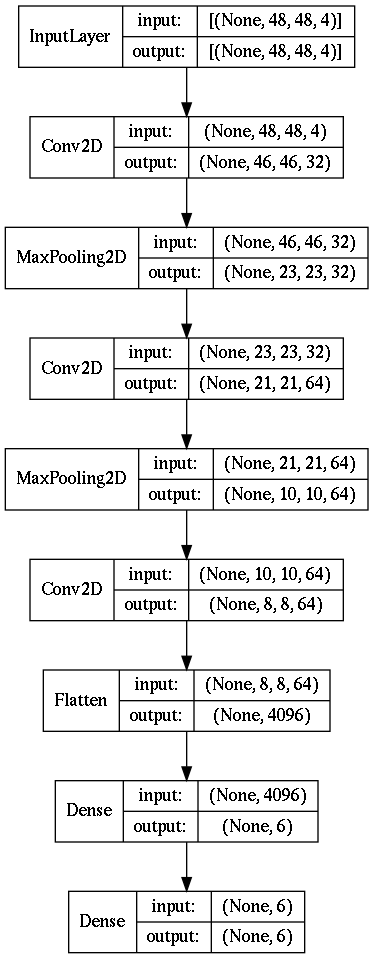
\includegraphics[height=0.9\linewidth]{images/model_cnn.png}
\caption{Basic model for prediction stage}
\label{fig:modelCNN}
\end{figure}

